\documentclass[12pt]{article}
\usepackage[margin=1in]{geometry} 
\usepackage{amsmath,amsthm,amssymb,amsfonts}
\usepackage{enumerate,listings,graphicx,epstopdf,siunitx}
\usepackage{bm}
\usepackage{color}
\graphicspath{~/Documents/school/fall16/stat586/hw8}
\setcounter{secnumdepth}{0}

\sloppy
\definecolor{lightgray}{gray}{0.5}
 
\newcommand{\N}{\mathbb{N}}
\newcommand{\Z}{\mathbb{Z}}
\newcommand{\normD}[3]{\frac{1}{\sqrt{2\pi #1^2}}exp\left(\frac{-( #2 - #3)^2}{2 #1^2}\right)} 
\newcommand{\cProb}[2]{P(#1|#2)}
\newcommand{\infSum}{\lim_{n\to\infty} \sum_{n=i}^\infty}

\begin{document}
\title{Homework Set 8}
\author{Taylor Bodin}
\maketitle

\section{Problem 7.9}
\subsection{a.}
\begin{align*}
  \lim_{n\to\infty} P\left( |S_n-S|^2 > \epsilon^2 \right) &\leq \lim_{n\to\infty} \frac{E[(s_n-s)^2]}{\epsilon^2} \\
  \lim_{n\to\infty} P\left( |S_n-S|^2 > \epsilon^2 \right) &\leq 0 \\
  \lim_{n\to\infty} P\left( |S_n-S| > \epsilon \right) &\leq 0 \\
  \lim_{n\to\infty} P\left( |S_n-S| > \epsilon \right) &= 0 & & \textrm{since probability cannot be negative.}
\end{align*}

\subsection{b.}
The cauchy distribution is the classic case where something can converge in probability and not in the MS sense. 

\section{Problem 7.11}
\subsection{a.}
A sequence of cauchy RVs of the form $\frac{X}{1+n^2}$ converges almost everywhere, but has no mean and therefore
cannot converge in the MS sense. Proof of this is shown in problem 7.13.

\subsection{b.}
Suppose a random sequence of $X\sim unif(1,2)$ with $\mu = 1.5$ is constructed such that 
$X_n = \lim_{n\to\infty} \sum_{i=1}^n X_i$. The random sequence does not converge, but will
converge in the MS sense since $S_n = \lim_{n\to\infty} \frac{1}{n} \sum_{i=1}^n X_i = \mu$. 

\section{Problem 7.13}
\subsection{Convergence Everywhere}
Since, $X \sim Cauchy$ its support is on $(-\infty,\infty)$.

\[
  X_n = 
\begin{cases}
  \lim_{n\to\infty} \frac{X}{1+n^2} = 0 & x \neq \infty \\ 
  \lim_{n\to\infty} \frac{X}{1+n^2} = \frac{\infty}{\infty} = undef & x = \infty
\end{cases}
\] 

Thus the sequence converges almost everywhere.

\subsection{Convergence in Probability and Distribution}
Convergence almost everywhere implies convergence in probability and distribution.

\subsection{Convergence in the MS sense}
\begin{align*}
  0 &= \lim_{n\to\infty} E\left[ |X_n|^2 \right] \\
  &= \lim_{n\to\infty} E\left[ \left(\frac{X}{1+n^2}\right)^2 \right] \\
  &= \lim_{n\to\infty} \frac{X}{(1+n^2)^2} E[ X^2 ] \to DNE
\end{align*}
This RV does not converge in MS sense. 

\section{Problem 7.15}
\subsection{Convergence Everywhere}

\[
  \lim_{n\to\infty} \sum_{i=0}^{\infty} \left( \frac{1}{2} \right)^{n-i} X_i =
  \lim_{n\to\infty} 2n\mu_X \nrightarrow 0
\] 

Thus the sequence does not converge.

\subsection{Convergence in Probability and Distribution}
Since the random sequence is composed of linear combinations of Gaussian RVs, the 
sequence itself is a Gaussian RV with some $\mu$ and $\sigma^2$
\[
  P(|S_n - \mu| > \epsilon) = 2Q\left( \sqrt{\frac{n\sigma}{\sigma^2}} \right)
\]

Then in the limit, the probability goes to 0 and the random sequence converges in
probability. This also implies convergence in distribution.

\subsection{Convergence in the MS sense}
\begin{align*}
  0 &= \lim_{n\to\infty} E\left[ |Z_n - \mu|^2 \right] \\
  &= \lim_{n\to\infty} Var(Z_n) \\
  &= \lim_{n\to\infty} \frac{\sigma^2}{n} \\
\end{align*}

The expression above does indeed equal zero and thus the random sequence converges in
the MS sense.

\section{Problem 7.17}

Since the random sequence is composed of linear combinations of Gaussian RVs, the 
sequence itself is a Gaussian RV with some $\mu$ and $\sigma^2$. Further, because
the sample mean is an unbiased estimator of the mean, as n approaches infinity
$S_n = \mu$. Therefore:

\[
  P(|S_n - \mu| > \epsilon) = P(0 > \epsilon) = 0
\]

The random sequence converges in probability which implies convergence in distribution.

\subsection{Convergence in the MS sense}
\begin{align*}
  0 &= \lim_{n\to\infty} E\left[ |S_n - \mu|^2 \right] \\
  &= \lim_{n\to\infty} Var(S_n) \\
  &= \lim_{n\to\infty} E[S_n^2] - \mu^2 \\
  &= \lim_{n\to\infty} E\left[\left(\frac{1}{n}\sum_{i=1}^n X_i\right)^2\right] - \mu^2 \\
  &= \lim_{n\to\infty} E\left[\frac{1}{n^2}\sum_{i=1}^n\sum_{j=1}^n X_iX_j\right] - \mu^2 \\
  &= \lim_{n\to\infty} \frac{1}{n^2}\sum_{i=1}^n\sum_{j=1}^n E\left[X_iX_j\right] - \mu^2 \\
  &= \lim_{n\to\infty} \frac{1}{n^2}\sum_{i=1}^n\sum_{j=1}^n \left(Cov(X_i,X_j) + \mu^2 \right) - \mu^2 \\
  &= \lim_{n\to\infty} Cov(X_i,X_j) + \mu^2 - \mu^2 \\
  &= \lim_{n\to\infty} \rho^{|k-m|}
\end{align*}

Since $\rho$ is strictly less than 1, the limit goes to 0 and thus the random sequence converges in the
MS sense. 

\section{Problem 7.19}
\subsection{a.}
\begin{align*}
  \Theta_{X}(\omega) &= E\left[ exp(j\omega X) \right] \\
  \Theta_{S_n}(\omega) &= E\left[ exp(j\omega\sum X) \right] \\
  &= E\left[ exp(j\omega X_1) \right]E\left[ exp(j\omega X_2) \right]E\left[ exp(j\omega X_3) \right] \cdots
  E\left[ exp(j\omega X_n) \right] \\
  &= \left(\Theta_X\left(\frac{\omega}{n}\right)\right)^n & \textrm{since X IID} 
\end{align*}

\subsection{b.}
\begin{align*}
  \Theta_X(\omega) &= \Theta_X(0) + \Theta_X^\prime(0)\omega + R_2(\omega) \\
   &= 1 + j\mu\omega + 0 \\
   c_0 &= 1 \\
   c_1 &= j\mu\omega
 \end{align*}

 \subsection{c.}
 \begin{align*}
   \Theta_{S_n}(\omega) &= \lim_{n\to\infty} \left( 1 + j\mu\frac{\omega}{n} + r_2\left( \frac{\omega}{n} \right) \right)^n \\
   &= \lim_{n\to\infty} \left( 1 + j\mu\frac{\omega}{n} \right)^n \\
   &= \infSum \binom{n}{i} \left( j\mu\frac{\omega}{n} \right)^k \\
   &= exp(j\mu\omega)
 \end{align*}

\section{Problem 7.21}
Let the sample means of the IID RVs be $X_i$. Then the mean of the sample means, $\mu$, can estimated by:
\[S_n = \frac{1}{n}\sum_{i=0}^n X_i\]
Because $S_n$ is an unbaised estimator for $\mu$, it will converge to that mean in the limit. Therefore
\[\lim_{n\to\infty}E\left[ \left( S_n - \mu \right)^2 \right] = 0\]
For this to be true, $E[X_i]$ must exist and $S_n$ must be an unbiased estimator of $\mu$. 

\section{Problem 7.23}
Since $X\sim u\left[ \frac{-1}{\sqrt{12}},\frac{1}{\sqrt{12}} \right]$, it has mean 0 and variance $\frac{1}{36}$.

\begin{align*}
  Z &= \frac{1}{\sqrt{n}} \sum_{i=1}^n \frac{X_i}{\sqrt{1/36}} \\
  Z &= \frac{6}{\sqrt{n}} \sum_{i=1}^n X_i \\
  S_n &= \sum_{i=1}^n X_i \\
  Z &= \frac{6}{\sqrt{n}} S_n \\
  Z &\sim N(0,1)
\end{align*}

\section{Problem 7.25}
Since $X\sim binom(1,0.02)$, the mean will be $np = .02$ and the variance will be $np(p-1) = .0196$.
\begin{align*}
  Z_n &= \frac{1}{\sqrt{1023}} \sum_{i=1}^{1023} \frac{X_i-.02}{\sqrt{.0196}} \\
  &= \frac{1}{\sqrt{1023}} \frac{S_n-(1023).02}{\sqrt{.0196}} \\
  &= \frac{1}{\sqrt{1023}} \frac{30-(1023).02}{\sqrt{.0196}} \\
  &= 2.131 \\
  P(X<30) &= P(Z<2.131) = 1- Q(2.131) = 98.35 \%
\end{align*}

\section{Problem 7.27}
\subsection{a.}
\[
  P\left( \sum_{k=1}^n X_k >y \right) \leq \frac{E\left[ \sum X \right]}{y} = \frac{n}{y}
\]
\subsection{b.}
\[
  P(\sum_{k=1}^n X_k > y) \leq P(\big|\sum_{k=1}^n X_k - n\big| > y-n) \leq \frac{Var(S_n)}{(y-n)^2} \leq \frac{n}{(y-n)^2}
\]
\subsection{c.}
\[
  P(\sum_{k=1}^n X_k > y) \leq \underset{s}{\text{min}} \ exp(-sy)M_Y(s) = exp(n-y)\left( \frac{y}{n} \right)^n
\]
\subsection{d.}
\begin{align*}
  \sum X_k &\sim N(n,n) \\
  P(\sum X_k > y) &= Q\left( \frac{y-n}{\sqrt{n}} \right)
\end{align*}
\subsection{e.}
\begin{align*}
  y &= \sum_{k=1}^n X_k \sim Erlang \\
  f_y(Y) &= \frac{y^{n-1}e^{-y}}{(n-1)!} \\
  P(y>Y) &= \int_y^\infty \frac{y^{n-1}e^{-y}}{(n-1)!} \\
\end{align*}
\subsection{f.}
\subsubsection{Log Space}
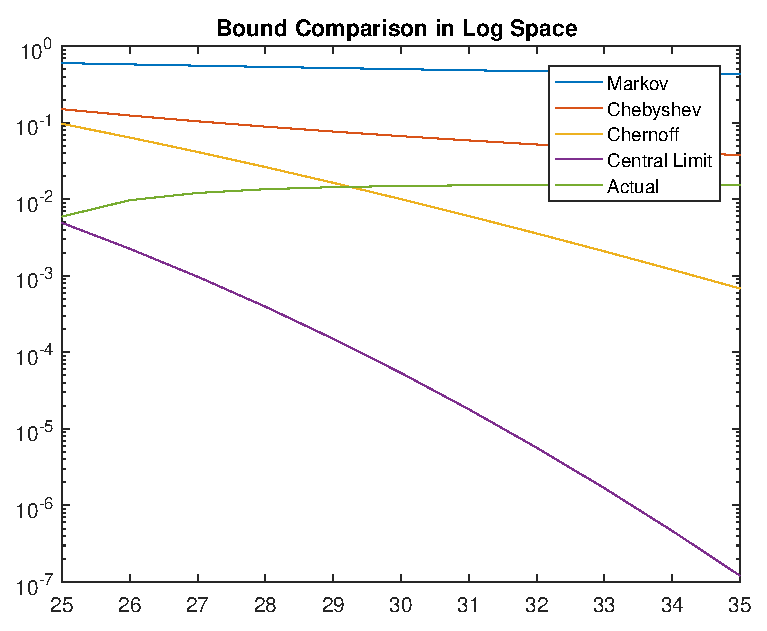
\includegraphics [width=4in]{prob7_27_01.eps}
\subsubsection{Linear Space}
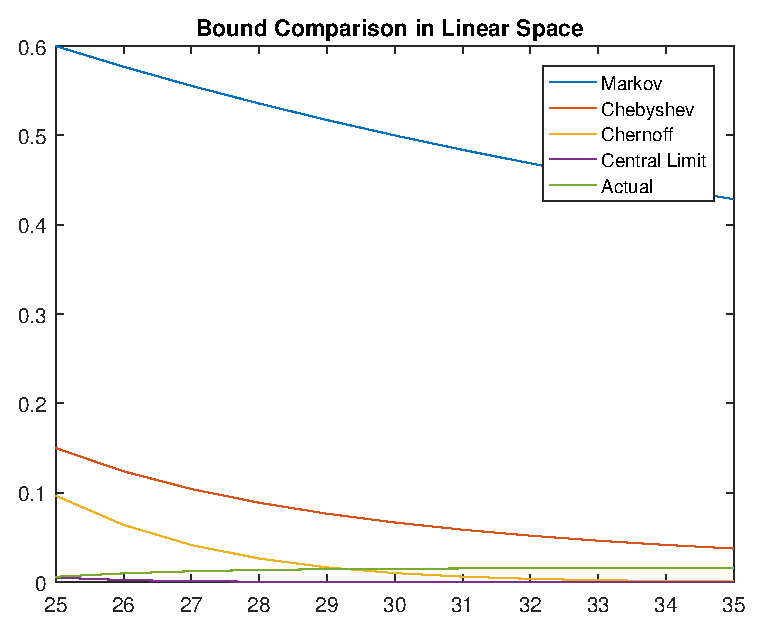
\includegraphics [width=4in]{prob7_27_02.eps}

\section{Problem 7.29}
Since $N\sim NBinom(m,p)$, the expected value of N is $m\left( \frac{1}{p} -1 \right)$. 
\subsection{a.}
\begin{align*}
  E[\hat P_A] &= E\left[ \frac{m-1}{N-1} \right] \\
  &= \frac{m-1}{E[N]-1} \\
  &= \frac{m-1}{m\left( \frac{1}{p} -1 \right)-1} \\
  &= \frac{m-1}{\frac{m}{p} -m -1} \neq p \\
\end{align*}
Thus the estimator is biased. 

\subsection{b.}
\begin{align*}
  E[\hat P_A] &= E\left[ \frac{m}{N} \right] \\
  &= \frac{m}{E[N]} \\
  &= \frac{m}{m\left( \frac{1}{p} -1 \right)} \\
  &= \frac{m}{\frac{m}{p} -m} \neq p \\
\end{align*}
Thus the estimator is biased. The estimator $\frac{m}{N+m}$ should work. 

\section{Problem 7.31}
\begin{align*}
  \epsilon_a &= \frac{\sigma_X}{\sqrt{N_1}} Q^{-1}(.1/2) \\
  \epsilon_a &= \frac{\sigma_X}{\sqrt{N_2}} Q^{-1}(.001/2) \\
  \frac{\sigma_X}{\sqrt{N_1}} Q^{-1}(.1/2) &= \frac{\sigma_X}{\sqrt{N_2}} Q^{-1}(.001/2) \\
  N_2 &= N_1\left( \frac{Q^{-1}(.001/2)}{Q^{-1}(.1/2)} \right)^2 \\
  N_2 &= N_1\left( \frac{3.29}{1.64} \right)^2 \\
  N_2 &= 4.024N_1
\end{align*}

\subsection*{Contents}

\begin{itemize}
\setlength{\itemsep}{-1ex}
   \item Problem 7.43
   \item Set up RVs
   \item Plots
\end{itemize}


\subsection*{Problem 7.43}

\begin{verbatim}
clear; close all; clc;
\end{verbatim}


\subsection*{Set up RVs}

\begin{verbatim}
N=1000000; % Set number of samples
z=[0:0.1:20]; % define variable for horizontal axis
w=randn(3,N).*4 + 3; % generate uniform random samples
W = sqrt(w(1,:).^2 + w(2,:).^2 + w(3,:).^2);
F=zeros(1,length(z)); % initialize CDF estimate
for n=1:N % estimate CDF
F=F+(W(n)<z);
end
F=F/N;
\end{verbatim}


\subsection*{Plots}

\begin{par}
CDF
\end{par} \vspace{1em}
\begin{verbatim}
figure(1)
plot(z,F) % plot results
xlabel('x'); ylabel('F_X(x)')

% PDF
figure(2)
fx = diff(F);
plot(z(1:end-1),fx)
xlabel('x'); ylabel('f_X(x)')
\end{verbatim}

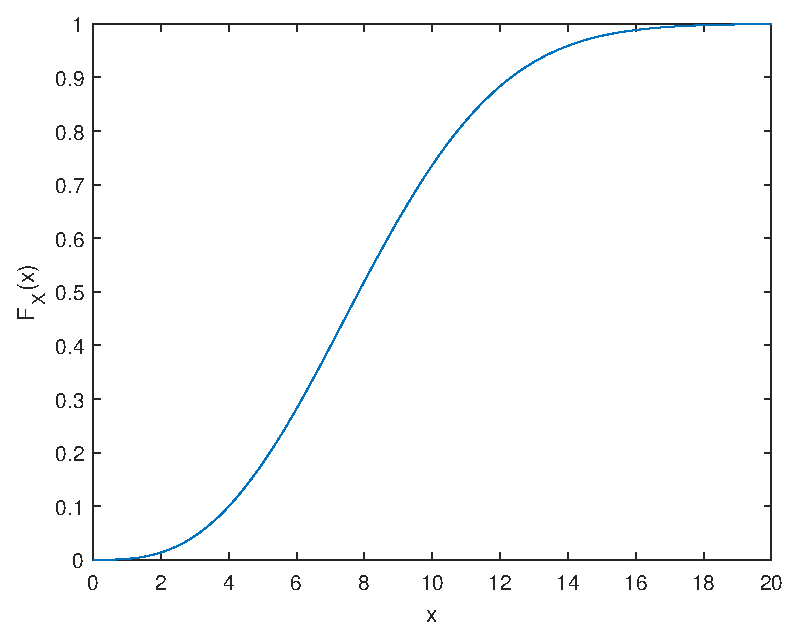
\includegraphics [width=4in]{prob7_43_01.eps}

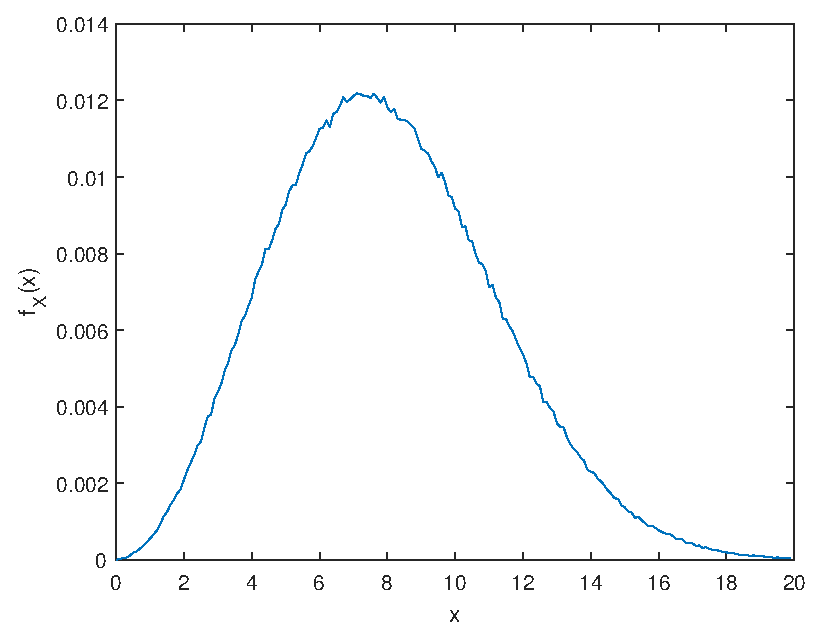
\includegraphics [width=4in]{prob7_43_02.eps}

\end{document}
